\begin{apendicesenv}

%\partapendices

\chapter{Questionário de Pesquisa}
\label{ap:questionario}

Este apêndice mostra as perguntas do questionário (Tabela \ref{tab:quest-survey}), instrumento de coleta usado na pesquisa com \textit{survey}. 

\begin{table} [!h]
\centering
\caption{Perguntas do Questionário de Pesquisa}
\label{tab:quest-survey}
\begin{tabular}{|p{16cm}|}
\hline

\textbf{Seção do Questionário - Dados Demográficos} \\ \hline

I01 - Qual é a sua idade? \\ \hline

I02 - Qual o seu sexo? \\ \hline

I03 - Qual o nome da sua instituição de ensino? \\ \hline

I04 - Meu curso de graduação é da área Ciência da Computação? \\ \hline

\textbf{Seção do Questionário - Habilidades e Competências} \\ \hline

O01 - Em relação à disciplina de Interação Humano-Computador (IHC):\\ \hline

H01 - Qual sua experiência com design de interfaces de software ou aplicativos?
\\ \hline

H02 -  Quais as atividades você já exerceu no processo de design de interfaces?
\\ \hline

H03 - Sobre o uso da técnica de personas:
\\ \hline

RL01 - O que você costuma fazer para sanar as dúvidas sobre algum conteúdo?
\\ \hline

O02 - Você já usou jogos para aprender algum conteúdo?\\ \hline

\textbf{Seção do Questionário - Perfil do usuário que jogava } \\ \hline

O02.1.1 - Quais motivos levaram você a usar esse tipo de jogo? \\ \hline

O02.1.2 - Com qual frequência você usava esse tipo de jogo? \\ \hline

O02.1.3 - Cite alguns jogos para aprendizagem que você já utilizou? \\ \hline

O02.1.4 - Quais motivos levaram você a deixar de usar esse tipo de jogo? \\ \hline

\textbf{Seção do Questionário - Perfil do Usuário que Joga  } \\ \hline

O02.2.1 - Quais motivos levaram você a usar esse tipo de jogo?\\ \hline

O02.2.2 - Com qual frequência você usava esse tipo de jogo?\\ \hline

O02.2.3 - Cite alguns jogos para aprendizagem que você  utiliza atualmente?\\ \hline

\textbf{Seção do Questionário - Perfil de usuário que nunca jogou  } \\ \hline

O02.3.1 - Quais motivos levariam você a usar esse tipo de jogo?\\ \hline

O02.3.2 Por que você nunca usou esse tipo de jogo?
\\ \hline

\textbf{Seção do Questionário - Perfil do usuário que não tem interesse } \\ \hline

O02.4.1 Por que você não tem interesse nesse tipo de jogo?\\ \hline

\textbf{Seção do Questionário - Caraterísticas de um jogo. Fatores de Usabilidade e Experiência do Jogador } \\ \hline

RE01  - Qual a relevância destes elementos para esse tipo de jogo?\tablefootnote{Os elementos da questão RE01  estão na Tabela \ref{tab:req-qualit}, com os indicadores de prioridade de 01 ao 12.} \\ \hline

E01 - Qual a importância destes elementos para uma boa experiência com estes jogos?\tablefootnote{Os elementos da questão E01 estão na Tabela \ref{tab:exp-player}, com os indicadores de prioridade de 01 ao 08.}\\ \hline

\end{tabular}

\end{table}

Este questionário segue uma lógica condicional a partir da questão O02. Ao optar por algumas das opções desta questão o respondente é encaminhado para uma ramificação distinta. Ao selecionar a opção ``Já usei, mas não jogo mais” o respondente é direcionado para questão O02.1.1; caso opte ``Eu uso” ele continua da questão O02.2.1; caso opte ``Não uso, mas tenho interesse em jogar” o respondente segue para questão O02.3.1, mas se optar por ``Não uso e não tenho interesse em jogar” ele é direcionado para O02.4.1. 

Dependendo da opção selecionada quando o participante da pesquisa responder a algumas destas questões O02.1.4, O02.2.3, O02.3.2 ou O02.4.1 o respondente continuará a responder a partir da questão RE01.


%-------------------Tabela RQ -------------------

Na Tabela \ref{tab:req-qualit} são apresentados os requisitos de qualidade apreciados pelos jogadores referentes aos item da questão RE01 da Tabela \ref{tab:quest-survey}.

\begin{table}[htbp]
\centering
\caption{Requisitos de Qualidade Apreciados pelos Jogadores}
\label{tab:req-qualit}
\begin{tabular}{clcl}
\hline
\multicolumn{1}{|c|}{\textbf{Identificador}} & \multicolumn{1}{l|}{\textbf{Requisito de Qualidade}} \\ \hline
\multicolumn{1}{|c|}{01}                  & \multicolumn{1}{l|}{\textit{Design} do jogo atraente} \\ \hline
\multicolumn{1}{|c|}{02}                  & \multicolumn{1}{l|}{Padrão de \textit{design} consistente}  \\ \hline
\multicolumn{1}{|c|}{03}                  & \multicolumn{1}{l|}{Facilidade em aprender a jogar}   \\ \hline
\multicolumn{1}{|c|}{04}                  & \multicolumn{1}{l|}{Facilidade em jogar}   \\ \hline
\multicolumn{1}{|c|}{05}                  & \multicolumn{1}{l|}{Regras fáceis e claras de se entender} \\ \hline
\multicolumn{1}{|c|}{06}                  & \multicolumn{1}{l|}{Fontes usadas serem fáceis de ler}   \\ \hline
\multicolumn{1}{|c|}{07}                  & \multicolumn{1}{l|}{Uso adequado das cores}   \\ \hline
\multicolumn{1}{|c|}{08}                  & \multicolumn{1}{l|}{Acessibilidade}  \\ \hline
\multicolumn{1}{|c|}{09}                  & \multicolumn{1}{l|}{Oferece \textit{feedback} ao jogador}           \\ \hline
\multicolumn{1}{|c|}{10}                  & \multicolumn{1}{l|}{Possui uma narrativa ou história}     \\ \hline
\multicolumn{1}{|c|}{11}                  & \multicolumn{1}{l|}{Oferece pontos e recompensas}    \\ \hline
\multicolumn{1}{|c|}{12}                  & \multicolumn{1}{l|}{Apresenta \textit{ranking} dos jogadores}  \\ \hline

\end{tabular}
\end{table}

%-------------------Tabela PX -------------------

Na Tabela \ref{tab:exp-player} são apresentados os requisitos de qualidade apreciados pelos jogadores referentes aos item da questão E01 da Tabela \ref{tab:quest-survey}.

\begin{table}[htbp]
\centering
\caption{ Experiência Apreciada pelos Jogadores}
\label{tab:exp-player}
\begin{tabular}{clcl}
\hline
\multicolumn{1}{|c|}{\textbf{Identificador}} & \multicolumn{1}{l|}{\textbf{Experiência apreciada pelos jogadores}}  \\ \hline
\multicolumn{1}{|c|}{1}                   & \multicolumn{1}{l|}{Ter confiança de que aprenderei o conteúdo}     \\ \hline
\multicolumn{1}{|c|}{2}                   & \multicolumn{1}{l|}{Me sentir desafiado}                  \\ \hline
\multicolumn{1}{|c|}{3}                   & \multicolumn{1}{l|}{Sentir satisfação em jogar e aprender}         \\ \hline
\multicolumn{1}{|c|}{4}                   & \multicolumn{1}{l|}{Interagir com outros jogadores}             \\ \hline
\multicolumn{1}{|c|}{5}                   & \multicolumn{1}{l|}{Me divertir}                                   \\ \hline
\multicolumn{1}{|c|}{6}                   & \multicolumn{1}{l|}{Ter a atenção focada durante o jogo}            \\ \hline
\multicolumn{1}{|c|}{7}                   & \multicolumn{1}{l|}{Perceber a relevância do conteúdo ensinado}      \\ \hline
\multicolumn{1}{|c|}{8}                   & \multicolumn{1}{l|}{O jogo como o principal meio de aprendizagem}        \\ \hline
                                                                                                    
\end{tabular}
\end{table}

A versão completa do questionário encontra-se no repositório: \url{https://github.com/RecursosDigitaisdeEnsinoAprendizagemIHC/research-pack-hci-games}.

%nas Figuras \ref{Fig:survey1.png}, \ref{Fig:survey2.png} e \ref{Fig:survey3.png}.

% \begin{figure}[htbp]
% 	\centering
% 	\subfigure[Questionário Parte 1]{
%         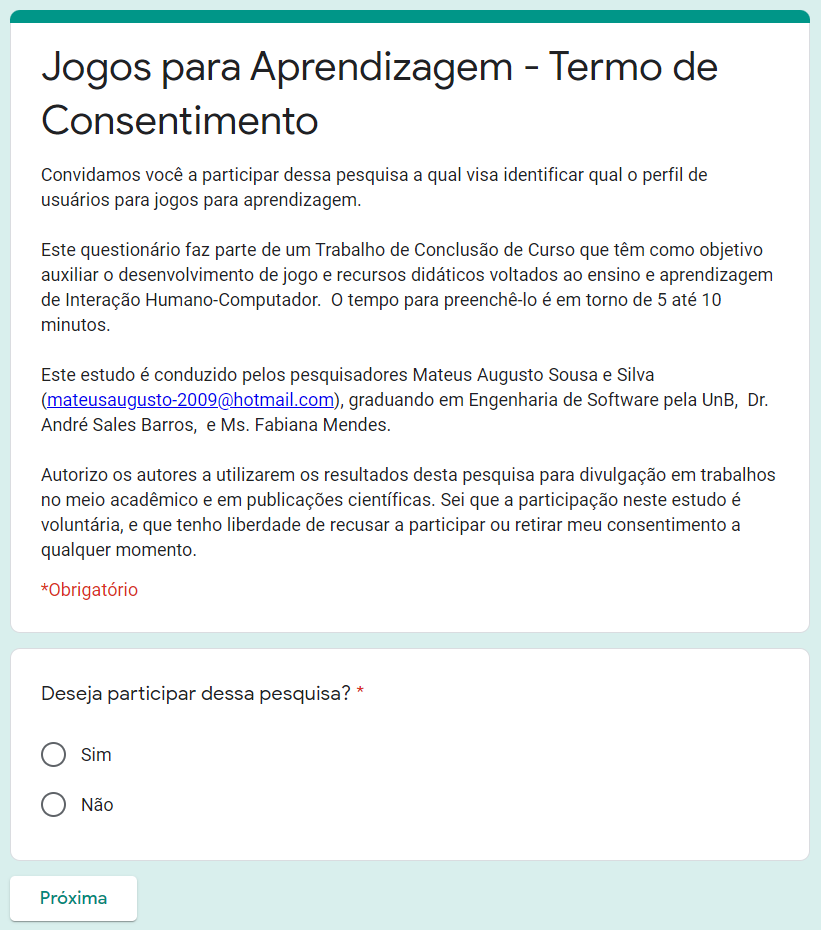
\includegraphics[keepaspectratio=true,scale=0.325]{figuras/apendice/Capture.PNG}
%         \label{Fig:survey_pt1.png}
%     }
%     \quad
%     \subfigure[Questionário Parte 2]{
%         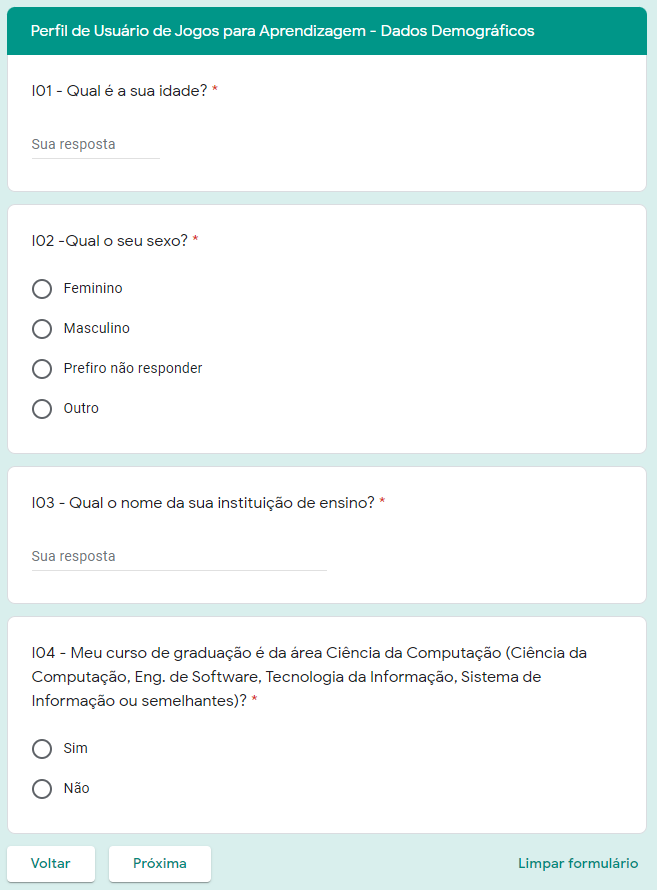
\includegraphics[keepaspectratio=true,scale=0.325]{figuras/apendice/Capture1.PNG}
%         \label{Fig:survey_pt2.png}
%     }
%     \quad
%      \subfigure[Questionário Parte 3]{
%         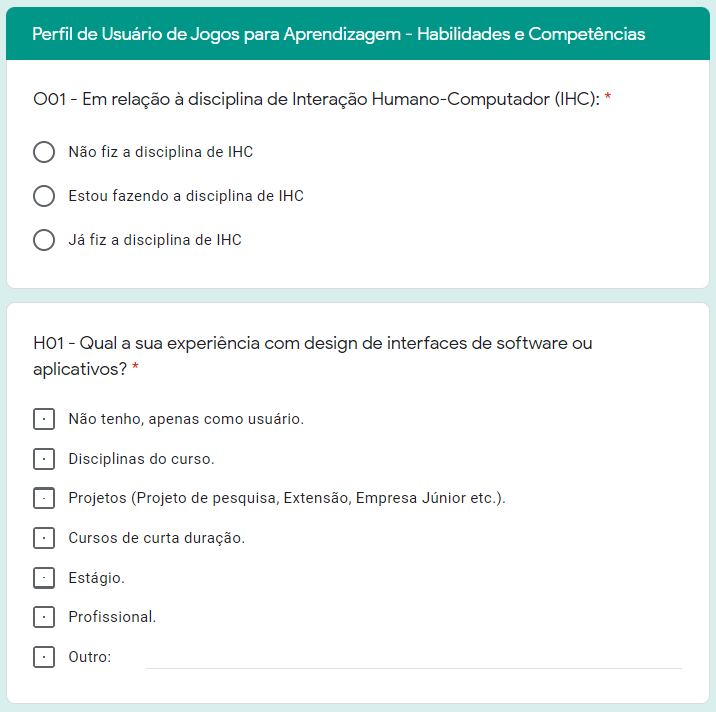
\includegraphics[keepaspectratio=true,scale=0.325]{figuras/apendice/Capture2.PNG}
%         \label{Fig:survey_pt3.png}
%     }
%     \quad
%      \subfigure[Questionário Parte 4]{
%         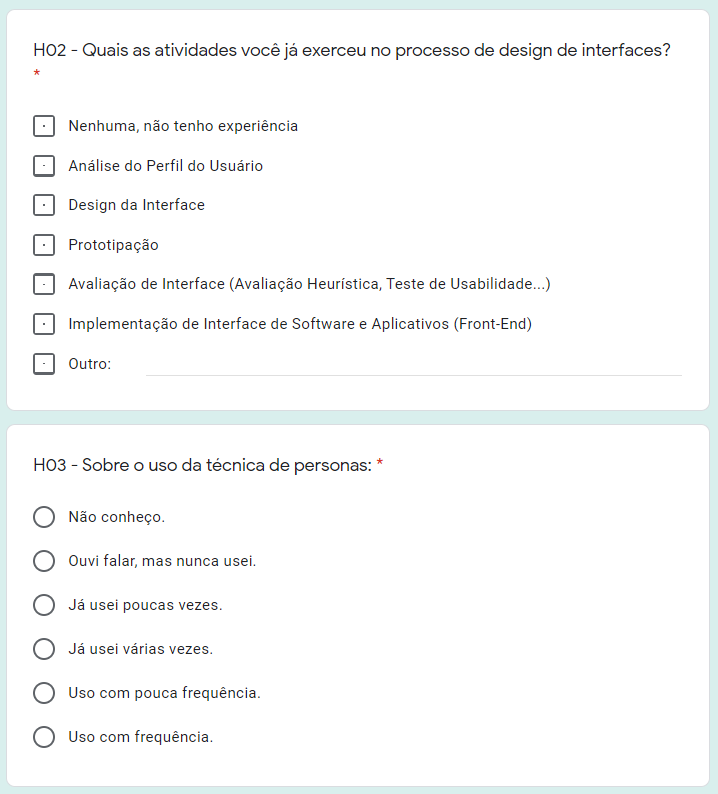
\includegraphics[keepaspectratio=true,scale=0.325]{figuras/apendice/Capture3.PNG}
%         \label{Fig:survey_pt4.png}
%     }
   
% 	\caption{Questionário de Pesquisa da Parte 1 à 4 - Fonte: Autoral}
% 	\label{Fig:survey1.png}
% \end{figure}

% \begin{figure}[htbp]
% 	\centering
% 	\subfigure[Questionário Parte 5]{
%         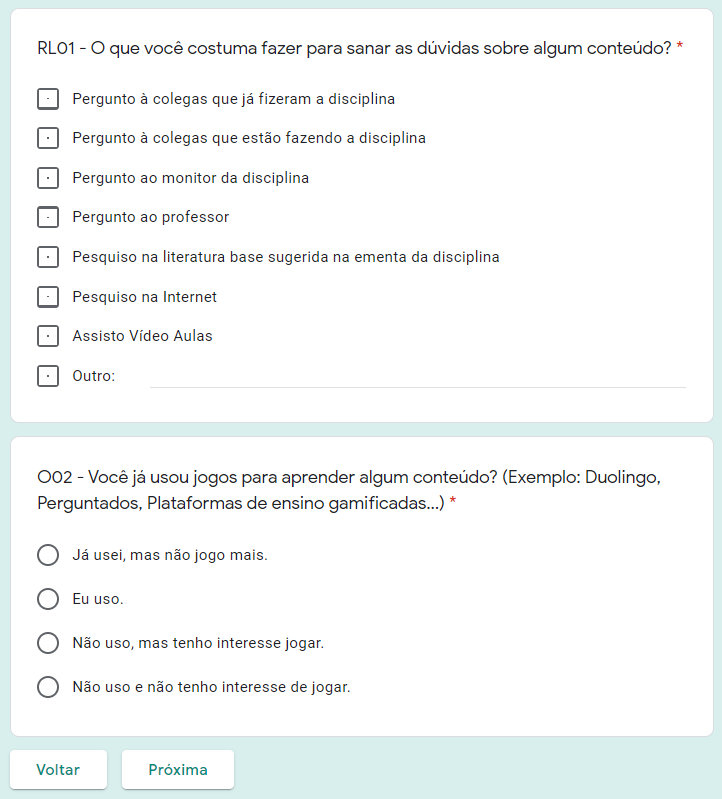
\includegraphics[keepaspectratio=true,scale=0.325]{figuras/apendice/Capture4.PNG}
%         \label{Fig:survey_pt5.png}
%     }
%     \quad
%     \subfigure[Questionário Parte 6]{
%         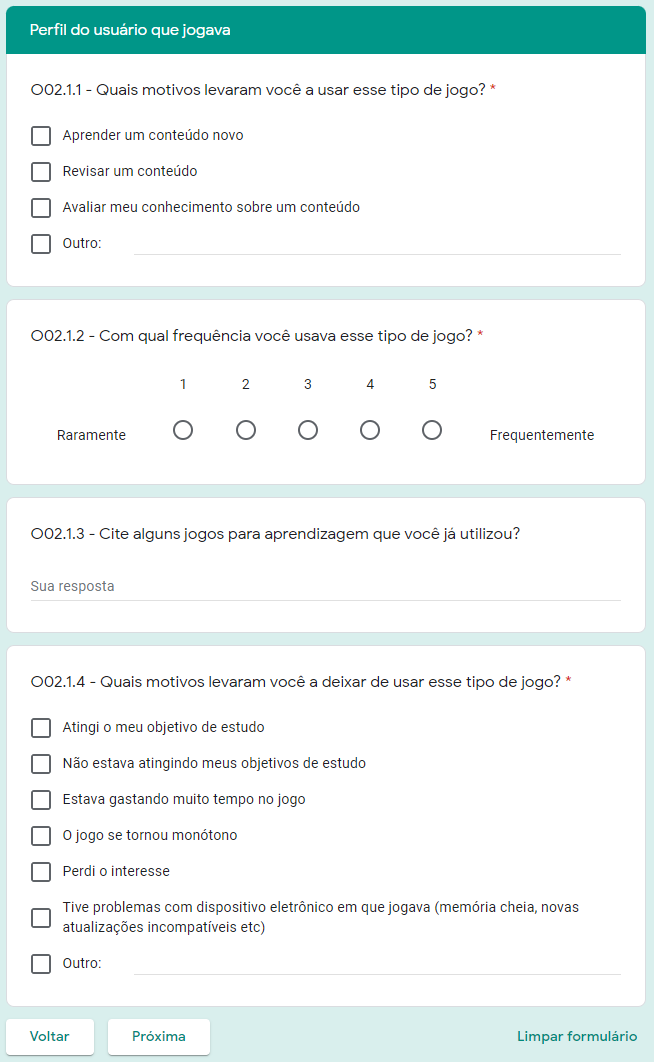
\includegraphics[keepaspectratio=true,scale=0.325]{figuras/apendice/Capture5.PNG}
%         \label{Fig:survey_pt6.png}
%     }
%     \quad
%      \subfigure[Questionário Parte 7]{
%         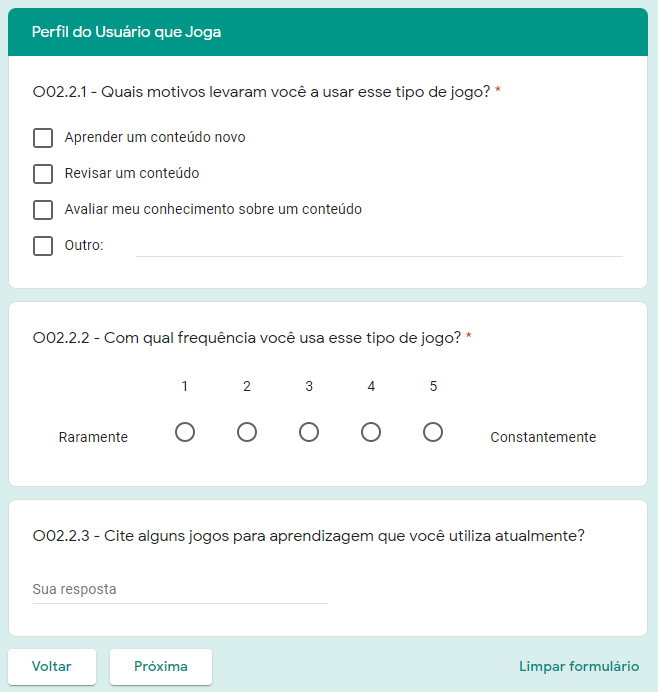
\includegraphics[keepaspectratio=true,scale=0.325]{figuras/apendice/Capture6.PNG}
%         \label{Fig:survey_pt7.png}
%     }
%     \quad
%      \subfigure[Questionário Parte 8]{
%         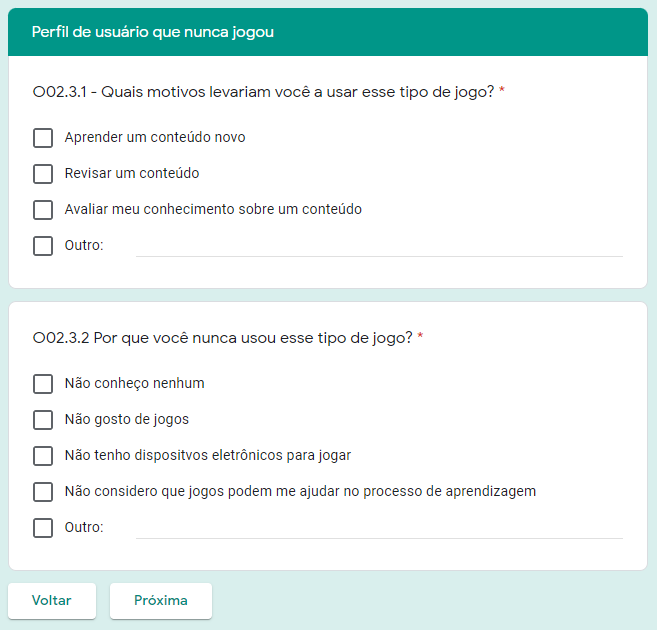
\includegraphics[keepaspectratio=true,scale=.325]{figuras/apendice/Capture7.PNG}
%         \label{Fig:survey_pt8.png}
%     }
   
% 	\caption{Questionário de Pesquisa da Parte 5 à 8 - Fonte: Autoral}
% 	\label{Fig:survey2.png}
% \end{figure}

% \begin{figure}[htbp]
% 	\centering
% 	\subfigure[Questionário Parte 9]{
%         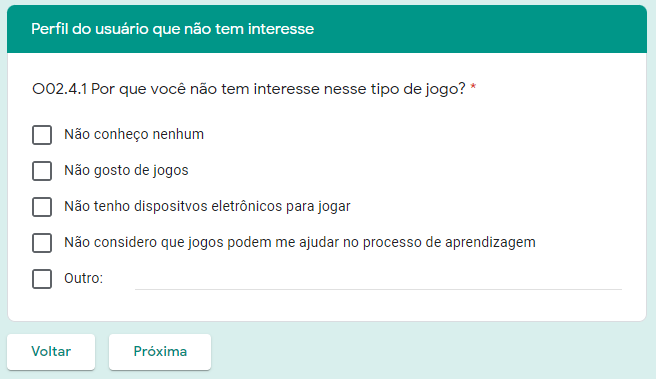
\includegraphics[keepaspectratio=true,scale=0.325]{figuras/apendice/Capture8.PNG}
%         \label{Fig:survey_pt9.png}
%     }
%     \quad
%     \subfigure[Questionário Parte 10]{
%         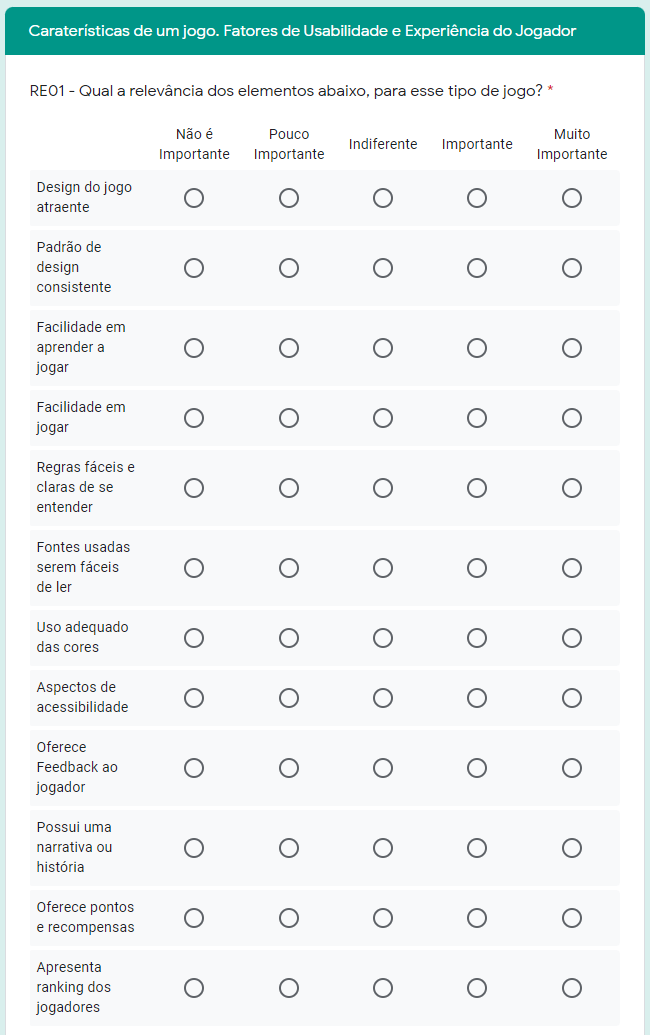
\includegraphics[keepaspectratio=true,scale=0.325]{figuras/apendice/Capture9.PNG}
%         \label{Fig:survey_pt10.png}
%     }
%     \quad
%      \subfigure[Questionário Parte 11]{
%         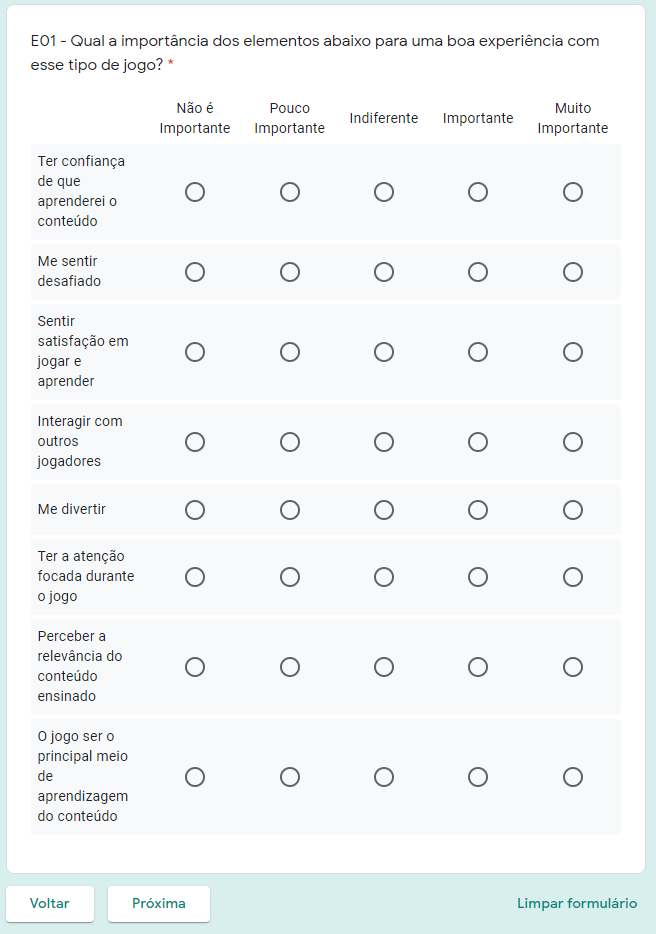
\includegraphics[keepaspectratio=true,scale=0.325]{figuras/apendice/Capture10.PNG}
%         \label{Fig:survey_pt11.png}
%     }
%     \quad
%      \subfigure[Questionário Parte 12]{
%         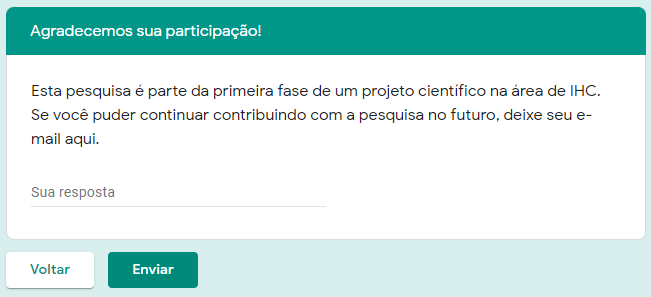
\includegraphics[keepaspectratio=true,scale=0.325]{figuras/apendice/Capture11.PNG}
%         \label{Fig:survey_pt12.png}
%     }
   
% 	\caption{Questionário de Pesquisa da Parte 9 à 12 - Fonte: Autoral}
% 	\label{Fig:survey3.png}
% \end{figure}


\end{apendicesenv}